% This is a LaTeX dvd menu design document autogenerated by dvdmenuauthor
%    from ex.dmp.xml at Sat Jan 14 16:11:41 2012
\def\autoloadXinputenc{\usepackage[latin2]{inputenc}}

\begingroup\catcode\string`@11
\global\def\write@genmpegattr#1{%
  \def\reserved@a{#1}%
  \immediate\write\@auxout{\expandafter\@gobble\string\%
    DVD genmpeg attr:\expandafter\strip@prefix\meaning\reserved@a}%
}%
\AtBeginDocument{\write@genmpegattr{--audio-codec=ac3}}%
\AtBeginDocument{\write@genmpegattr{--video-with=ffmpeg}}%
\endgroup
% TeX comment <nice>
\documentclass{article}

\usepackage{dvdmenu}
\usepackage{graphicx}
\usepackage{lmodern}
\usepackage{t1enc}
\usepackage{color}
\autoloadXinputenc
%\definecolor{dvdselectedcolor}{rgb}{0,1,0}
%\definecolor{dvdhighlightedcolor}{rgb}{0,0,1}
%\dvdbuttonframesep2pt

\begin{document}

\begin{dvdmenupage}{a,bb,ccc6}% LaTeX-generated menu 1
\thispagecolor{yellow}
\kern5ex
\leftskip3em \rightskip3em
\fontfamily{phv}\bfseries
vmgm main menu Hi!\par
\dvdtextbutton{a}{J�mp t� m\`en� 2}\par
\dvdtextbutton{bb}{J�mp t� m\`en� 4 W W W W W W W W W W W W W W W W W W W W W W W W W W W W W W W W W W}\par
\dvdtextbutton{ccc6}{J�mp t� m\`en� 6}\par
\end{dvdmenupage}

\begin{dvdmenupage}{a,bb,ccc}% LaTeX-generated menu 2
\thispagebgimage{}{pal_bg_light}
\vfil
\leftskip3em \rightskip3em
\hrule height0pt
\vskip-\parskip
\textbf{menu 2}\par
\dvdtextbutton{a}{J�mp t� m\"a\i n m\`en�}\par
\dvdtextbutton{bb}{J�mp t� m\`en� 2}\par
%\pdfliteral direct{1 0 0 1 -10000 -10000 cm}%
\dvdtextbutton{ccc}{J�mp t� m\`en� 3}
\hrule height0pt
\end{dvdmenupage}

\begin{dvdmenupage}{a,bb,ddd}% LaTeX-generated menu 3
\thispagebgimage{}{pal_bg_stripe2}
\kern5ex
\leftskip3em \rightskip3em
\textbf{menu 3}\par
\dvdtextbutton{a}{J�mp t� m\"a\i n
  \includegraphics{simple_button_back} m\`en�}\par
\color{red}
\dvdtextbutton{bb}{J�mp t� m\`en� 2}\par
%\color{dvdhighlightedcolor}
\color{blue}
\dvdtextbutton{ddd}{J�mp t� m\`en� 3}
\end{dvdmenupage}

\begin{dvdmenupage}{top,bottom}% LaTeX-generated menu 4
\kern5ex
\leftskip3em \rightskip3em
\textbf{menu 4, you aren't stuck here}\par
\par\noindent
  \dvdframebutton{top}{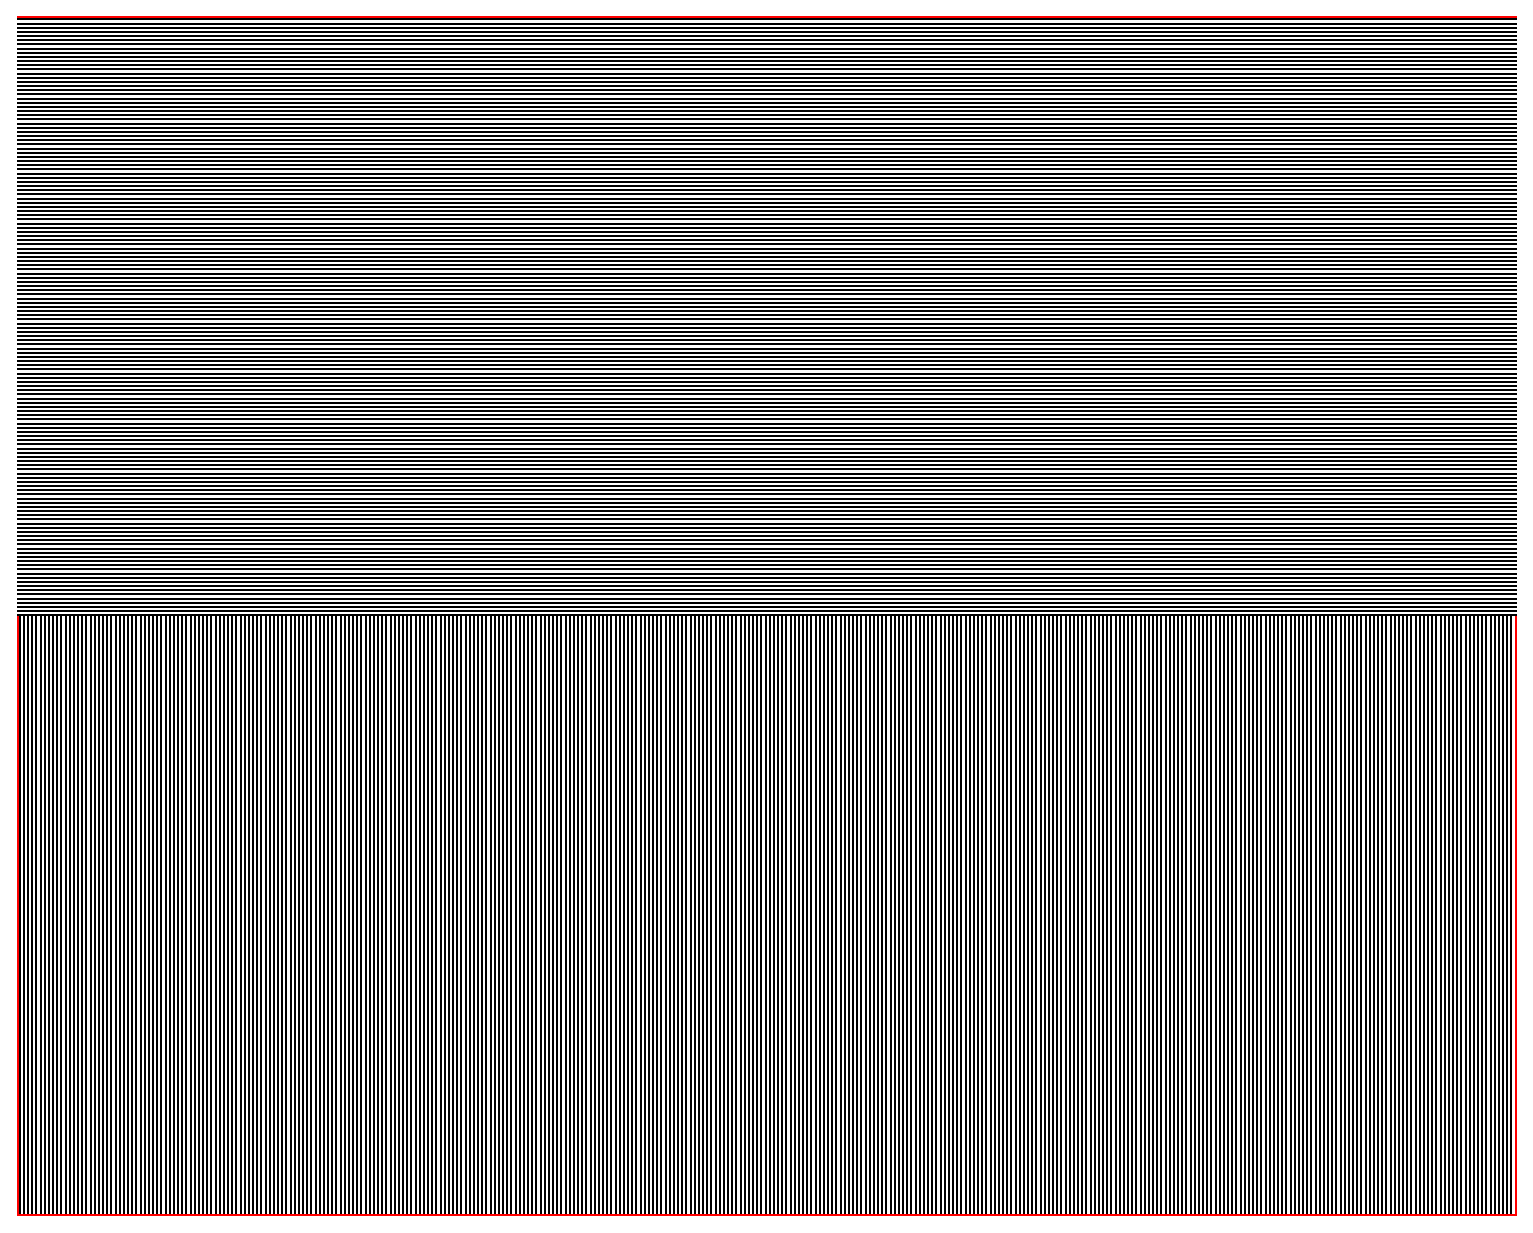
\includegraphics
    [width=.333333\paperwidth,height=.333333\paperheight]{pal_bg_stripe2}}
\par\noindent
  \dvdframebutton{bottom}{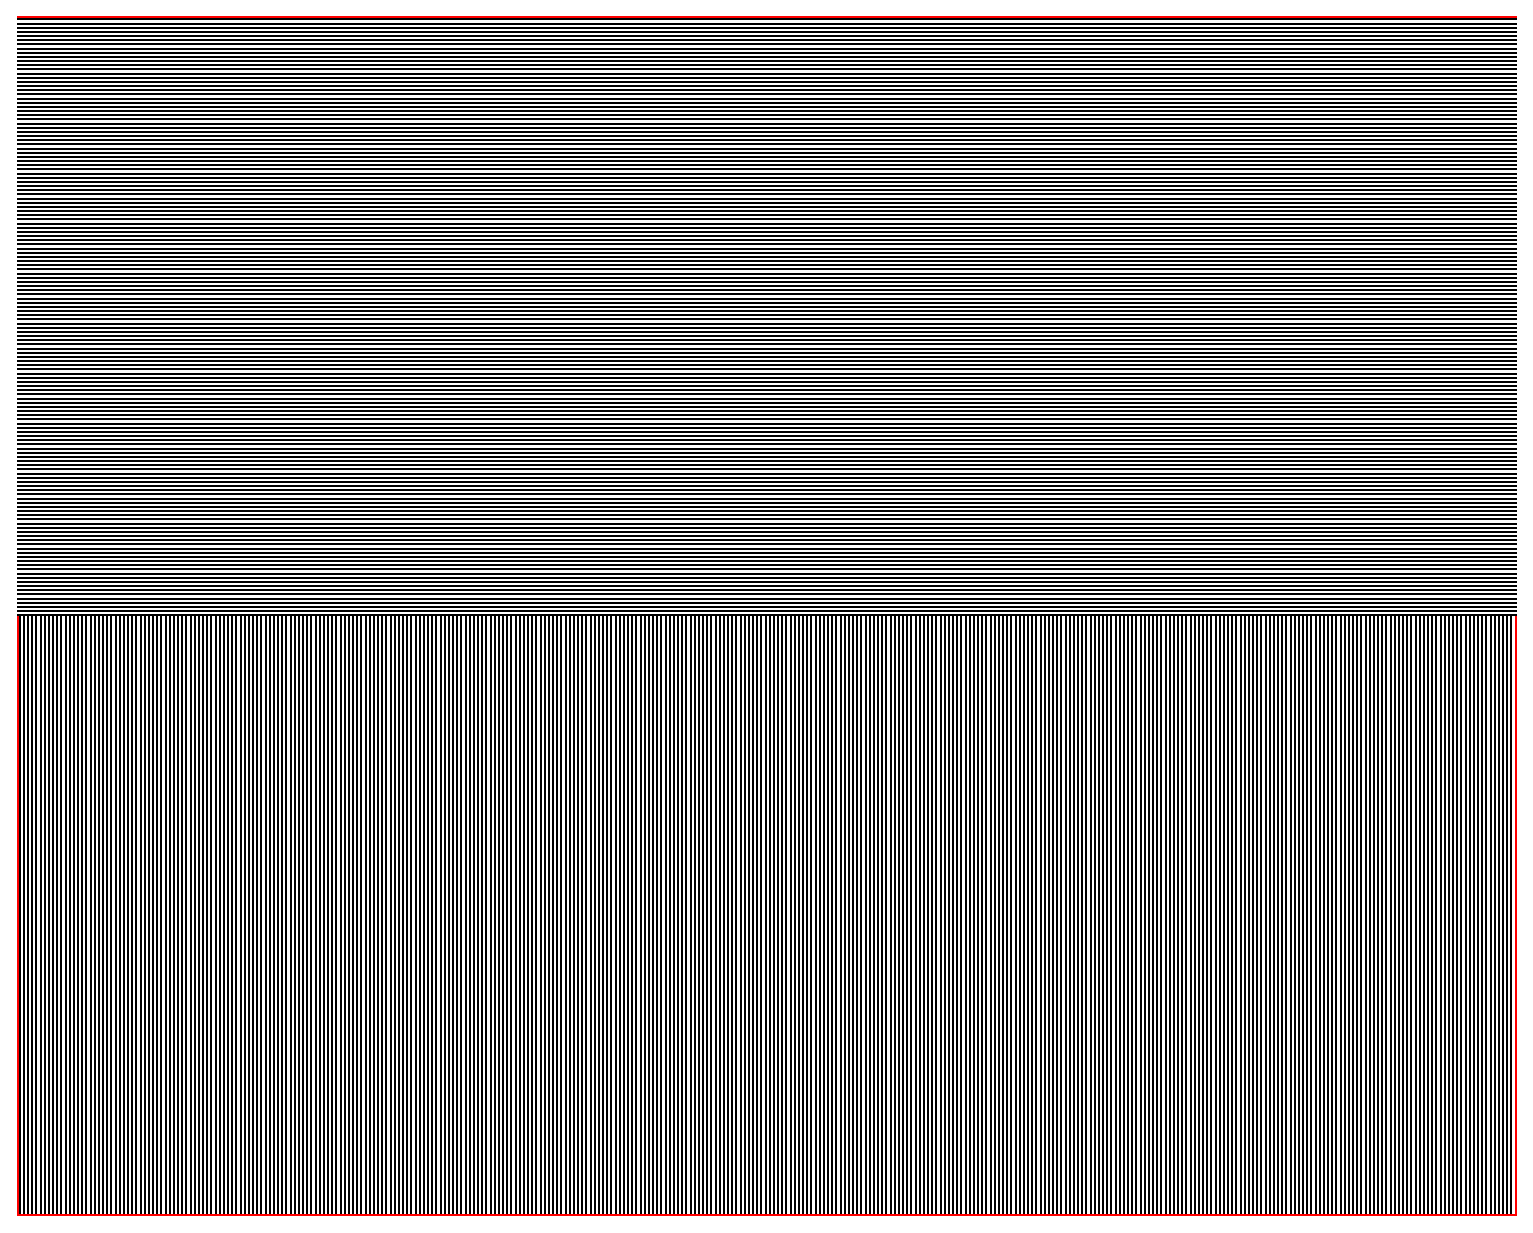
\includegraphics
    [width=.25\paperwidth,height=.25\paperheight]{pal_bg_stripe2}}
\end{dvdmenupage}

\begin{dvdmenupage}{}% LaTeX-generated menu 5
\kern5ex
\leftskip3em \rightskip3em
\textbf{menu 5, you are stuck here}\par
\par\noindent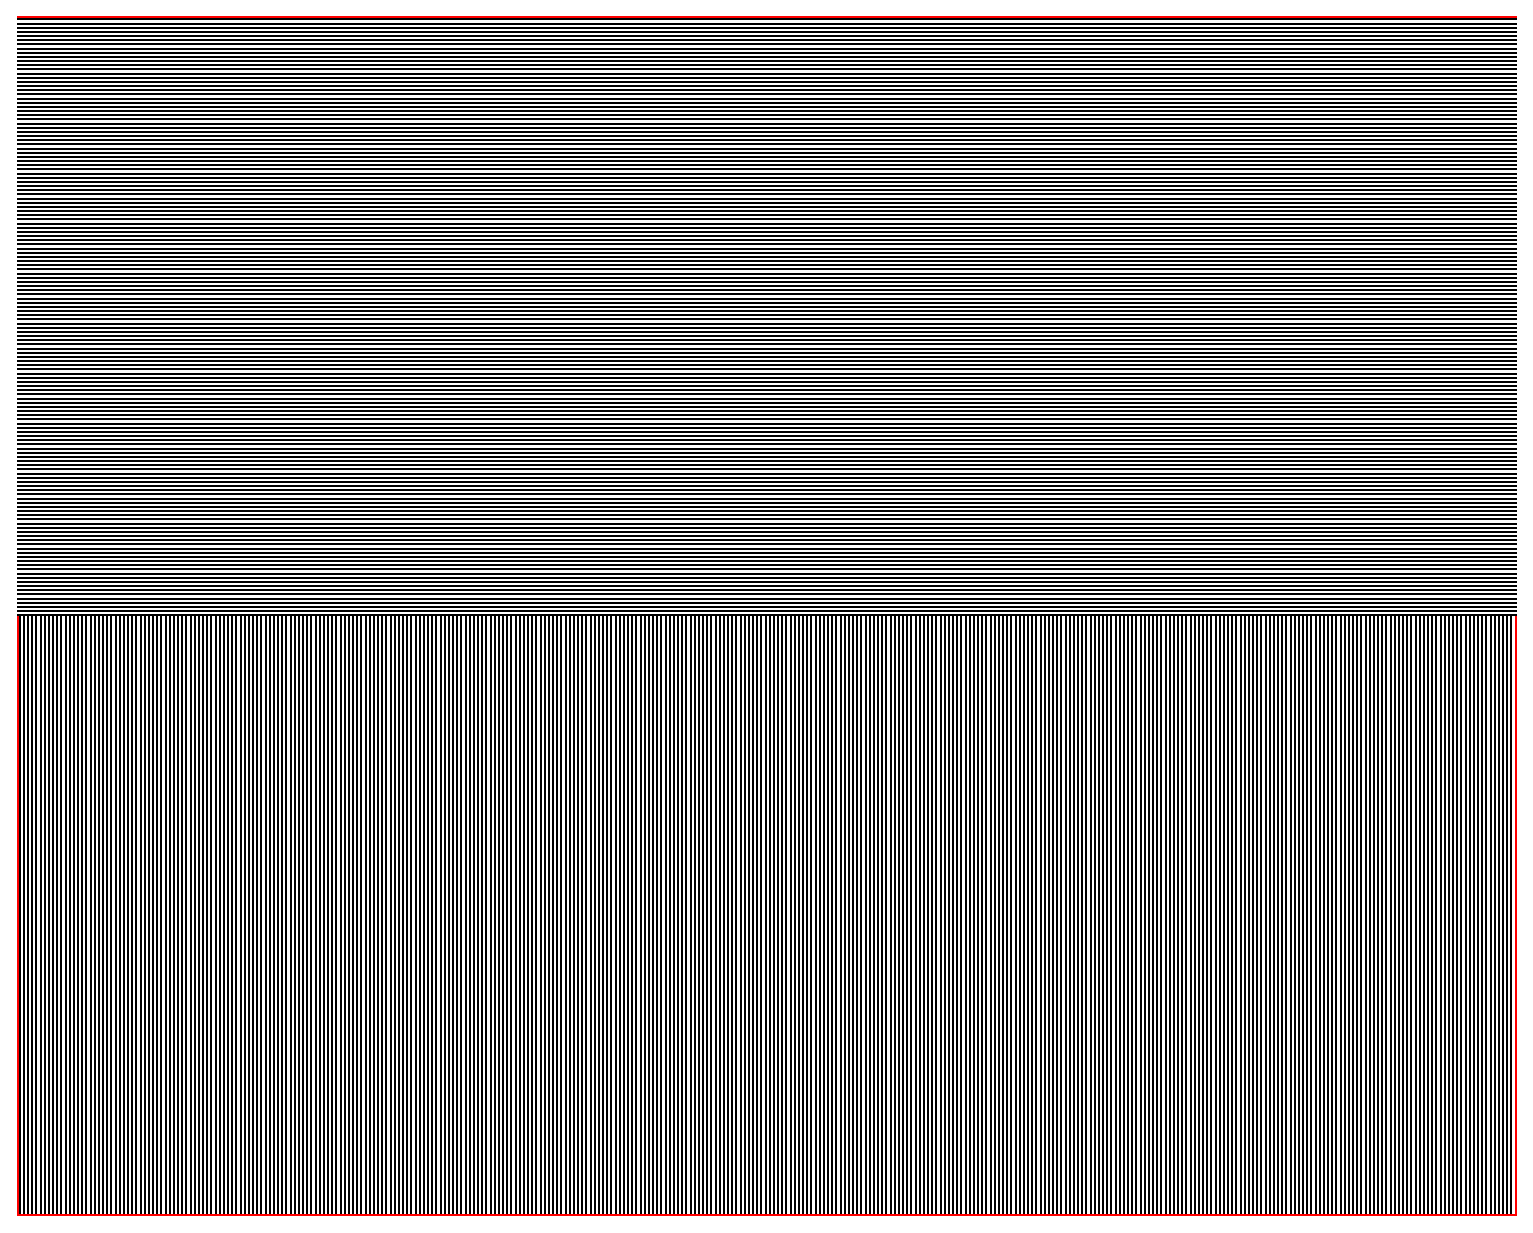
\includegraphics
  [width=.5\paperwidth,height=.5\paperheight]{pal_bg_stripe2}
\par\bigskip
\hrule height1.5bp
\end{dvdmenupage}

\begin{dvdmenupage}{e1,e2,e3,e4,e5,e6,prev,back,next}% LaTeX-generated menu 6
\thispagebgimage{}{pal_bg_light}
\thispagetemplate{palthumbsix}
\menucaption{Fazekas szalagavat� 1998.\ december}

\begingroup\def\dvdbuttonattrXname{e1}
  \def\dvdbuttonattrXcaption{a szalagt�z�s \emph{el�tt}}
  \def\dvdbuttonattrXimage{design/pal1.png}
\dvdprocessbutton\endgroup

\begingroup\def\dvdbuttonattrXname{e2}
  \def\dvdbuttonattrXcaption{szalagt�z�s}
  \def\dvdbuttonattrXimage{design/pal2.png}
\dvdprocessbutton\endgroup

\begingroup\def\dvdbuttonattrXname{e3}
  \def\dvdbuttonattrXcaption{oszt�lyt�ncok}
  \def\dvdbuttonattrXimage{design/pal3.png}
\dvdprocessbutton\endgroup

\begingroup\def\dvdbuttonattrXname{e4}
  \def\dvdbuttonattrXcaption{egy�b t�ncok}
  \def\dvdbuttonattrXimage{design/pal4.png}
\dvdprocessbutton\endgroup

\begingroup\def\dvdbuttonattrXname{e5}
  \def\dvdbuttonattrXcaption{vide�felv�telek}
  \def\dvdbuttonattrXimage{design/pal5.png}
\dvdprocessbutton\endgroup

\begingroup\def\dvdbuttonattrXname{e6}
  \def\dvdbuttonattrXcaption{keret}
  \def\dvdbuttonattrXimage{design/pal6.png}
\dvdprocessbutton\endgroup

\begingroup\def\dvdbuttonattrXname{prev}
  \def\dvdbuttonattrXdummy{}
\dvdprocessbutton\endgroup

\begingroup\def\dvdbuttonattrXname{back}
  \def\dvdbuttonattrXdummy{}
\dvdprocessbutton\endgroup

\begingroup\def\dvdbuttonattrXname{next}
  \def\dvdbuttonattrXdummy{}
\dvdprocessbutton\endgroup
\end{dvdmenupage}

% Bye!
\end{document}
